\documentclass[12pt, letterpaper]{article}

\usepackage[utf8]{inputenc}
\usepackage[english]{babel}
\usepackage[T1]{fontenc}
\usepackage{graphicx}
\usepackage{tikz}
\usepackage{subfig}
\usepackage{wrapfig}
\usepackage{longtable}
\usepackage{amsmath}
\newcommand\tab[1][1cm]{\hspace*{#1}}
\renewcommand{\baselinestretch}{1.3}

\begin{document}

\begin{titlepage}

\begin{center}
	\large{EC336: Embedded Systems}\\
	\huge{\textbf{Interfacing Display Devices}}\\
	\large{Arvind S Kumar (15EC106), Pavan M (15EC137),\\ Samarth B (15EC143), Sripathi M (15EC149)}\\
	\large{15 August 2018}
\end{center}	

\begin{figure}[!h]
	\centering
	\includegraphics[scale=0.8]{/home/sripathi/GitHub_Repositories/NITK_Emblem.png}
	\label{fig:NITKEmblem}
\end{figure}	
\begin{center}
	
\huge{Submitted to:}\\
\begin{large}
Prof. Ramesh Kini M, Prof. Arulalan Rajan\\
Department of Electronics and Communication Engineering\\
NITK, Surathkal
\end{large}

\end{center}

\end{titlepage}

\section{Goal of the Lab}

The aim of this lab was to interface the chosen microcontroller with display devices such as LEDs, 7-segment displays and LCD. The micro controller chosen by our group is TI's MSP430G2.

\section{Components Used}

For this lab the components used are :

\begin{itemize}
	\item MSP430 microcontroller
	\item LEDs
	\item 2.2 k$\Omega$ resistors
	\item 2 7-segment displays
	\item LCD
\end{itemize}

\section{Board Details}

Some of the features of the MSP430 are - (Refer Figure \ref{fig:architecture} and Figure \ref{fig:board} for more information)

\begin{itemize}
	\item 16-bit RISC architecture
	\item Von-Neumann architecture
	\item Upto 16 MHz clock frequency
	\item Low power consumption and five power saving modes
	\item 16 general purpose registers
	\item 10-bit ADC
	\item Supports SPI, I2C, UART and USB interfaces
	\item Has 16 GPIO pins divided as two ports (8-bit each)
\end{itemize}
	
\begin{figure}[t]
	\centering
	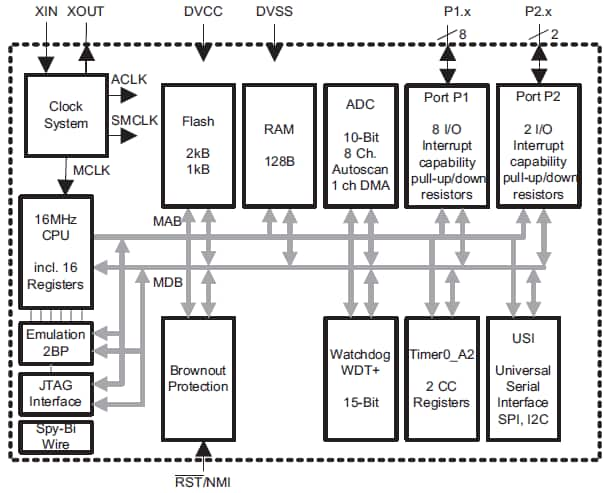
\includegraphics[scale=0.8]{/home/sripathi/GitHub_Repositories/Embedded-Systems/LatexFiles/msp430g2231-ep-ti.png}
	\caption{MSP430 Architecture}
	\label{fig:architecture}
\end{figure}

\begin{figure}[t]
	\centering
	\subfloat[fig:board][Board]{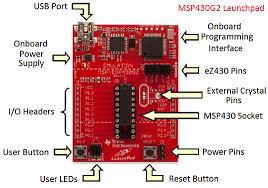
\includegraphics[scale=0.8]{/home/sripathi/GitHub_Repositories/Embedded-Systems/LatexFiles/board_msp430.jpeg}}
		\subfloat[fig:pindiagram][Pin Diagram]{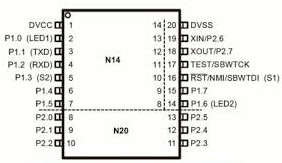
\includegraphics[scale=0.8]{/home/sripathi/GitHub_Repositories/Embedded-Systems/LatexFiles/pinout_msp430.jpeg}}
		\caption{Board details}
		\label{fig:board}
\end{figure}

\section{Interfacing Details}

Three display devices - LEDs, 7-segment displays and an LCD display were interfaced. The details for each of them are as follows - 

\subsection{LEDs}

To do this, first the on-board LEDs (LED1 and LED2) were made to blink using the given example program. LED1 is connected to Port 1 BIT0 and LED2 is connected to Port 2 BIT6.\\
To blink an external LED, we connected an LED through a 2.2k resistor to Port 1 BIT4.\\
The delays were controlled using do...while loops

\begin{figure}[!h]
	\centering
	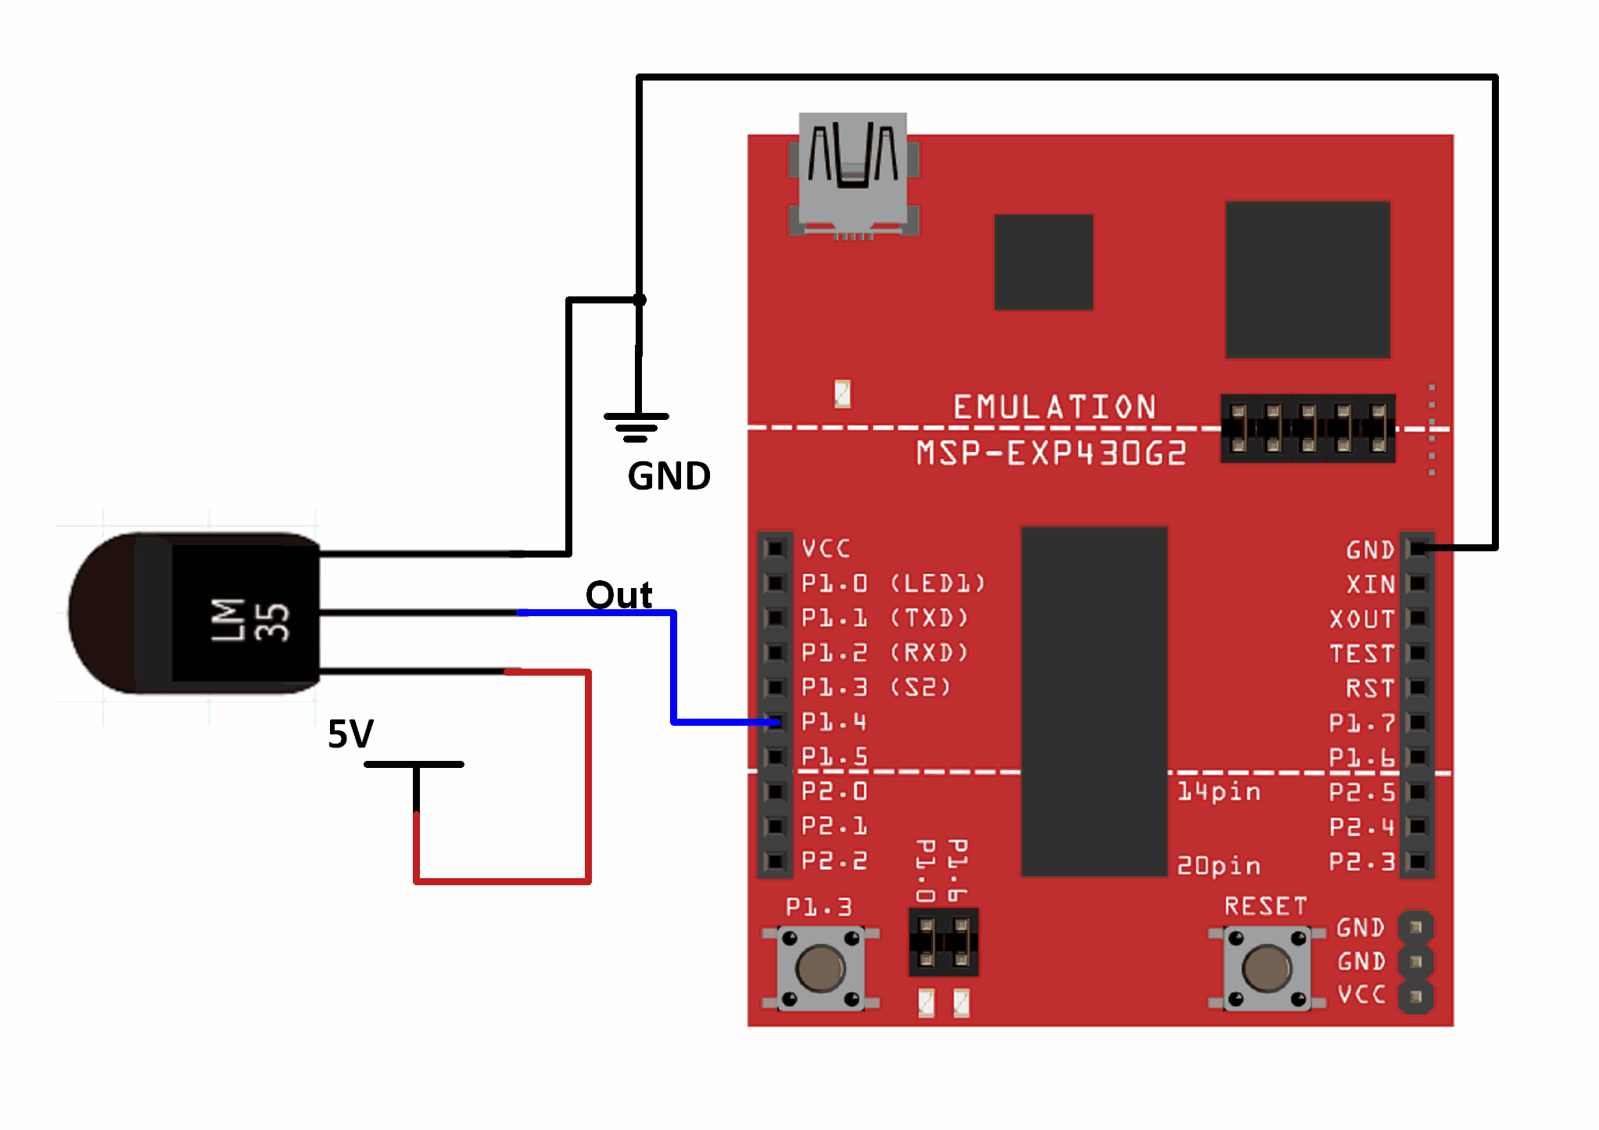
\includegraphics[scale=0.1, angle=270]{/home/sripathi/GitHub_Repositories/Embedded-Systems/LatexFiles/Interfacing_Display_Devices/LM35_Interfacing_Diagram.png}
	\caption{LED interface}
	\label{fig:ledInterface}
\end{figure}

\subsection{7-Segment Display}

\begin{wrapfigure}{r}{0.4\textwidth}
	\centering
	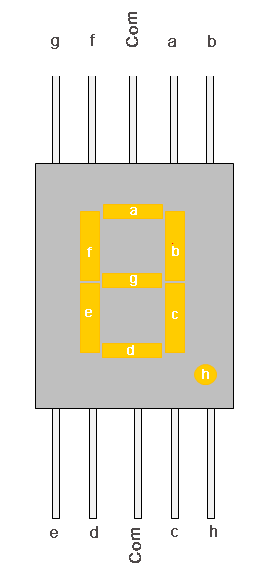
\includegraphics[width=0.28\textwidth]{/home/sripathi/GitHub_Repositories/Embedded-Systems/LatexFiles/Interfacing_Display_Devices/Seven-Segment-Display.png}
	\label{fig:7segment}
	\caption{7-Segment Display}
\end{wrapfigure}

To interface the 7-segment display, an array of the 7-segment 8 bit patterns were created and stored. A loop is run through these values and a delay is provided using do...while loops to be able to observe the transition. All 8 pins of Port 1 were used to interface the 7-segment display (including the decimal point)\\
Next, a two digit counter was made to count from 0 to 99. Both the 7-segment displays were connected to the same data lines (i.e Port 1) and to switch between the two displays the COM ports of the displays were controlled using a signal. This signal was generated using multiplexing between two bits on Port 2. By controlling the amount of delay, we were able to generate the illusion of a two digit counter.

\subsection{LCD}

The LCD was interfaced in the 4-bit 2-line configuration. The LCD was connected to the MSP430 as shown. 4 pins from Port 1 (BIT0 to BIT3) were connected to the LCD data pins D7-D4. The EN and RS pins of the LCD were connected to BIT4 and BIT5 of Port 1 respectively. Since we only want to write to the LCD, the RW pin of the LCD was grounded. To control the contrast, the contrast pin of the LCD was connected to a potential divider created using 4 2.2 k$\Omega$ resistors in a 3:1 configuration. The VCC and VSS pins of the LCD were connected to the 5V supply of the MSP430 (T1) and ground respectively. These help control the intensity of the back light.

\begin{figure}[!h]
	\centering
	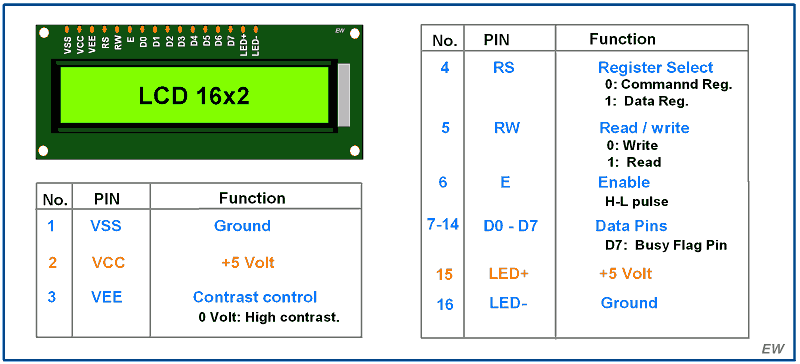
\includegraphics[scale=0.5]{/home/sripathi/GitHub_Repositories/Embedded-Systems/LatexFiles/Interfacing_Display_Devices/lcd_pins_new.png}
	\caption{LCD PIN diagram}
	\label{fig:lcdPinout}
\end{figure} 

\begin{figure}[!h]
	\centering
	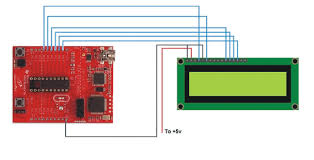
\includegraphics[scale=0.8]{/home/sripathi/GitHub_Repositories/Embedded-Systems/LatexFiles/Interfacing_Display_Devices/lcdInterface.jpeg}
	\caption{LCD interface}
	\label{fig:lcdInterface}
\end{figure} 

In order to print a message that is in infinite scroll on the LCD screen, a string with the message was used. Each chunk of 16 characters was sent to the LCD after a specific delay which was controlled using the delaycycles() command. At each iteration the first character of the 16 character chunk was removed and added to the end of the string.
\newpage
\section{Program}

%\begin{center}
\begin{longtable}{|p{6cm}||p{5cm}|}
%\caption{A sample long table.} \label{tab:long} \\

\hline 
\multicolumn{1}{|c|}{\textbf{Scanning of 7-Segment Display using MSP430}} & \multicolumn{1}{c|}{\textbf{Pseudo code}}  \\ 

%Scanning of 7-Segment Display using MSP430  & Pseudo code \\
\hline 
\endfirsthead

\multicolumn{2}{c}%
{{\bfseries \tablename\ \thetable{} -- continued from previous page}} \\
\hline 
%\multicolumn{1}{|c|}{\textbf{First column}} & \multicolumn{1}{c|}{\textbf{Second column}} & \multicolumn{1}{c|}{\textbf{Third column}} \\ 
\hline 
\endhead

\hline \multicolumn{2}{|r|}{{Continued on next page}} \\ \hline
\endfoot

\hline \hline
\endlastfoot



\#include <msp430.h>  & \\             
\#include <stdio.h>   &  \\

int main(void)\{ & \\

   \hspace{0.1cm} WDTCTL $=$  WDTPW $|$ WDTHOLD;    & Stop watchdog timer \\ 

    
  \hspace{0.1cm}  P1DIR $|=$ 0xff;    & Set all to output direction \\ 
  \hspace{0.1cm}  P2DIR $|=$ 0x03;       & set pin 2 to output direction for turning one of 7 segment on \\                 
  \hspace{0.1cm}  for(;;) \{   &  Begin loop\\
     \hspace{0.3cm}   long i; & \\   

     \hspace{0.3cm}   int segment[10] $=$ \{0xfc, 0x60, 0xd2, 0xf2, 0x66, 0xb6, 0xbe, 0xe0, 0xfe, 0xf6\}; & \\
      \hspace{0.3cm}  int var, loop; & \\

      \hspace{0.3cm}  for(var $=$ 0; var<100; var$++$) \{ & Count 0 to 99\\
        \hspace{0.5cm}    int seg1 $=$ segment[var/10]; & selecting 10's place\\ 
        \hspace{0.5cm}    int seg2 $=$ segment[var\%10]; & selecting 1's place \\
         \hspace{0.5cm}   i $=$ 10000; & \\
         \hspace{0.5cm}   do \{ & \\
            \hspace{0.5cm}    P2OUT $=$ 0x02; & \\
            \hspace{0.5cm}    P1OUT $=$ 0xFF \^ seg1; & turn on tens place and ones place off\\
            \hspace{0.5cm}    int j $=$ 100; &  delay \\
            \hspace{0.5cm}   do j$--$; & \\
            \hspace{0.5cm}    while(j $!=$ 0); & \\
            \hspace{0.5cm}    P1OUT $=$ 0xFF;    & turning of all leds of 7 segment \\
            \hspace{0.5cm}     j $=$ 100; & delay\\
            \hspace{0.5cm}    do j$--$; & \\
            \hspace{0.5cm}    while(j $!=$ 0); & \\
            \hspace{0.5cm}    P2OUT $=$ 0x01; & \\
            \hspace{0.5cm}    P1OUT $=$ 0xFF \^ seg2;     &  turn on ones place and turn off tens place\\
            \hspace{0.5cm}    j $=$ 100; & \\
            \hspace{0.5cm}    do j$--$; &  delay\\
            \hspace{0.5cm}    while(j $!=$ 0); & \\

            \hspace{0.5cm}    P1OUT $=$ 0xFF; & turning of all leds of 7 segment\\
            \hspace{0.5cm}    j $=$ 100; & \\
            \hspace{0.5cm}    do j$--$; & delay\\
            \hspace{0.5cm}    while(j $!=$ 0); & \\


             \hspace{0.5cm}   i$--$; & \\
          \hspace{0.5cm}  \}while(i $!=$ 0); &  Repeat again for some time\\
       \hspace{0.3cm} \}

  \hspace{0.1cm} \}
   
\}

\end{longtable}
%\end{center}
\newpage

\begin{longtable}{|p{6cm}||p{5cm}|}
%\caption{A sample long table.} \label{tab:long} \\

\hline 
\multicolumn{1}{|c|}{\textbf{Scrolling LCD Display using MSP430}} & \multicolumn{1}{c|}{\textbf{Pseudo code}}  \\ 

%Scanning of 7-Segment Display using MSP430  & Pseudo code \\
\hline 
\endfirsthead

\multicolumn{2}{c}%
{{\bfseries \tablename\ \thetable{} -- continued from previous page}} \\
\hline 
%\multicolumn{1}{|c|}{\textbf{First column}} & \multicolumn{1}{c|}{\textbf{Second column}} & \multicolumn{1}{c|}{\textbf{Third column}} \\ 
\hline 
\endhead

\hline \multicolumn{2}{|r|}{{Continued on next page}} \\ \hline
\endfoot

\hline \hline
\endlastfoot



\#include <msp430g2553.h> & \\
\#include <string.h> & \\


\#define lcdPort \hspace{0.5cm}        P1OUT & Defining ports \\
\#define lcdPortDir \hspace{0.5cm}    P1DIR & \\

\#define lcdEN      BIT4 & \\
\#define lcdRS      BIT5 & \\

void lcdReset() & function to reset\\
\{ &\\
        \hspace{0.1cm} lcdPortDir $=$ 0xff; &    setting pins to output mode \\
        \hspace{0.1cm} lcdPort $=$ 0xff;  &  \\
        \hspace{0.1cm} \_\_delay\_cycles(20000);  & delay \\

\} & \\

void lcdCmd (char cmd) & \\
\{ & \\
        
        \hspace{0.1cm} lcdPort $=$ ((cmd $>>$  4) \& 0x0F)$|$lcdEN; & Send upper nibble \\
        \hspace{0.1cm} lcdPort $=$ ((cmd $>>$ 4) \& 0x0F); & \\

       
        \hspace{0.1cm} lcdPort $=$ (cmd \& 0x0F)$|$lcdEN; & Send lower nibble \\
        \hspace{0.1cm} lcdPort $=$ (cmd \& 0x0F); & \\

        \hspace{0.1cm} \_\_delay\_cycles(4000);
\} & \\

void lcdInit () & \\
\{ & \\
        \hspace{0.1cm} lcdReset(); & Call LCD reset\\
        \hspace{0.1cm} lcdCmd(0x28);   &     4-bit mode \- 2 line \- 5x7 font.\\
        \hspace{0.1cm} lcdCmd(0x0C);   &     Display no cursor - no blink. \\
        \hspace{0.1cm} lcdCmd(0x80);   &     Address DDRAM with 0 offset 80h.\\
        \hspace{0.1cm} lcdCmd(0x01);   &     Clear screen \\
\} & \\


void lcdData (unsigned char dat) & Send the Data to LCD\\
\{ & \\
       
       \hspace{0.1cm} lcdPort $=$ (((dat $>>$ 4) \& 0x0F)$|$lcdEN$|$lcdRS); & Send upper nibble by right shifting the dat 4 four so we get the upper 4 bits\\
       \hspace{0.1cm} lcdPort $=$ (((dat $>>$ 4) \& 0x0F)$|$lcdRS); & \\

        
       \hspace{0.1cm} lcdPort $=$ ((dat \& 0x0F)$|$lcdEN$|$lcdRS); & Send lower nibble\\
       \hspace{0.1cm} lcdPort $=$ ((dat \& 0x0F)$|$lcdRS); & \\

        \hspace{0.1cm} \_\_delay\_cycles(4000); &  a small delay \\
\} & \\

void displayLine(char *line) & Function to Display the Character \\
\{ & \\
        \hspace{0.1cm} while (*line) & \\
         \hspace{0.3cm} lcdData(*line$++$); & Call lcdData function\\
\} & \\

int main() & \\
\{ & \\
        
        \hspace{0.1cm} WDTCTL $=$ WDTPW $+$ WDTHOLD; & Stop Watch Dog Timer\\

        
        \hspace{0.1cm} lcdInit(); & Initialize LCD\\
        
        
         \hspace{0.1cm} char name[] $=$ "EC336 EMBEDDED SYSTEMS "; & \\
        \hspace{0.1cm} int len $=$ strlen(name); & Get the length of the string\\
        \hspace{0.1cm} int j $=$ 0,i,k,c; & \\
        \hspace{0.1cm} char sub[16]; & \\
        
        
        \hspace{0.1cm} while(1)\{ & Start loop\\
          \hspace{0.3cm}      c $=$ 0; & \\
          \hspace{0.3cm}    lcdCmd(0x80); & \\
                
                
 
          \hspace{0.1cm} while (c < 16) & getting a substring of 16 characters\\
               \hspace{0.3cm} \{ & \\
                 \hspace{0.5cm} sub[c] $=$ name[j+c]; & \\
                  \hspace{0.5cm} c$++$;&\\
               \hspace{0.1cm} \}
                
                
 
             \hspace{0.1cm}   char var $=$ name[j]; & \\
             \hspace{0.1cm}   k $=$ 0; & \\
              \hspace{0.1cm}  while(k<len-1) & shifting all the characters left by one and putting the first character to the end \\
             \hspace{0.3cm}   \{ & \\
              \hspace{0.5cm}          name[k] $=$ name[k+1]; & \\
              \hspace{0.5cm}         k$++$; & \\
               \hspace{0.1cm} \} & \\
                \hspace{0.1cm} name[len-1] $=$ var; & \\
               \hspace{0.1cm}  name[len] $=$ '$\backslash$0'; & \\
              \hspace{0.1cm}  sub[c] $=$ '$\backslash$0'; & \\
             \hspace{0.1cm}   displayLine(sub); & Calling display function to print on lcd\\
             \hspace{0.1cm}   \_\_delay\_cycles(500000); & After small delay repeat the loop\\


        \} & \\


        while (1); & \\
\} & \\

\end{longtable}

\section{Knowledge Gained}

\begin{enumerate}
    \item Exposure to a new micro-controller platform. None of us had used MSP430 before neither in our hobby projects nor in course projects and hence it was a new learning experience.
    \item Shift in using in-built commands to register manipulation during programming resulted in a new learning curve.
    \item Understanding how an LCD is configured internally and trying to interface it with the controller and the logic employed to get a scrolling display.
    \end{enumerate}

\end{document}
